% Drawing 69/06-10 -- folder 69, batch 06, archive page 117 (PDF page 118).
% Transcription: un pentagone en forme de maison, partagé en triangles par des diagonales, quelques-unes fléchées
% Kind: house-shaped pentagon cut into triangles. Method 2 (schematic redraw from the facsimile). Status: partial.
% Notes: A pentagon shaped like a house, cut into triangles by diagonals, some with arrows. Which diagonals carry arrows is a reading.
% Coordinates: 1 unit = 1 mm = 1/100 of the crop width (bbox in page fractions: [0.52, 0.57, 0.66, 0.68]).
% Redrawn by Claude (claude-opus-5-5), issue #73, 2026-11-07; not checked by a human; not compiled (no TeX in the session).
% Rights: reproduces part of the work -- behind RENDER_TRANSCRIPTS, never published by itself.
\documentclass[tikz,border=3pt]{standalone}
\usepackage{amsmath,amssymb}
\usetikzlibrary{patterns,arrows.meta}
\tikzset{pencil/.style={black!45}, struck/.style={black!35}, mark/.style={circle,draw,inner sep=1.3pt}, pt/.style={circle,fill,inner sep=0.9pt}, opt/.style={circle,draw,fill=white,inner sep=1.1pt}}
\begin{document}
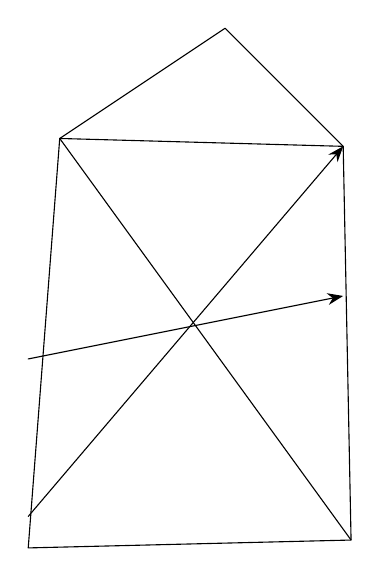
\begin{tikzpicture}[x=1mm,y=1mm,line cap=round,line join=round,font=\scriptsize]
\draw (49,-26) -- (64,-41) -- (65,-91) -- (24,-92) -- (28,-40) -- cycle;
\draw (28,-40) -- (64,-41);
\draw[-{Stealth[length=2mm]}] (24,-68) -- (64,-60);
\draw[-{Stealth[length=2mm]}] (24,-88) -- (64,-41);
\draw (28,-40) -- (65,-91);
\end{tikzpicture}
\end{document}
